\chapter{Figures}
\label{ch:figures}

\section{Image Files}
\label{sec:figures-image-files}

\begin{figure}[p]
	\centering
	\begin{minipage}[b]{0.70\textwidth}
		\includegraphics[width=\linewidth]{example-image}
	\end{minipage}
	\caption{Normal figure with a centered image file.}
	\label{fig:figures-normal}
\end{figure}

\begin{sidewaysfigure}
	\centering
	\begin{minipage}[b]{0.70\textwidth}
		\includegraphics[width=\linewidth,clip=true,trim=1cm 1cm 1cm 1cm]{example-image}
	\end{minipage}
	\caption{Sideways figure with a clipped and trimmed image file.}
	\label{fig:figures-sideways}
\end{sidewaysfigure}

\clearpage
\section{Multi-Panel Figures}
\label{sec:figures-multi-panel}

\begin{figure}[p]
	\centering
	\begin{minipage}[b]{0.49\textwidth}
		\includegraphics[width=\linewidth]{example-image-a}
		\subcaption{First subfigure}
		\label{fig:figures-subfigure-a}
	\end{minipage}
	\hfill
	\begin{minipage}[b]{0.49\textwidth}
		\includegraphics[width=\linewidth]{example-image-b}
		\subcaption{Second subfigure}
		\label{fig:figures-subfigure-b}
	\end{minipage}
	\caption{Figure with subcaptions for related panels.}
	\label{fig:figures-subfigures}
\end{figure}

\begin{figure}[p]
	\centering
	\begin{minipage}[b]{0.49\textwidth}
		\includegraphics[width=\linewidth]{example-image-a}
		\caption{Left figure in a side-by-side layout.}
		\label{fig:figures-side-by-side-left}
	\end{minipage}
	\hfill
	\begin{minipage}[b]{0.49\textwidth}
		\includegraphics[width=\linewidth]{example-image-b}
		\caption{Right figure in a side-by-side layout.}
		\label{fig:figures-side-by-side-right}
	\end{minipage}
	\caption{Two independent figures placed on one line.}
	\label{fig:figures-side-by-side}
\end{figure}

\clearpage
\section{TikZ Diagrams}
\label{sec:figures-tikz}

\begin{figure}[!ht]
\centering
\begin{minipage}[t]{0.49\textwidth}
\centering
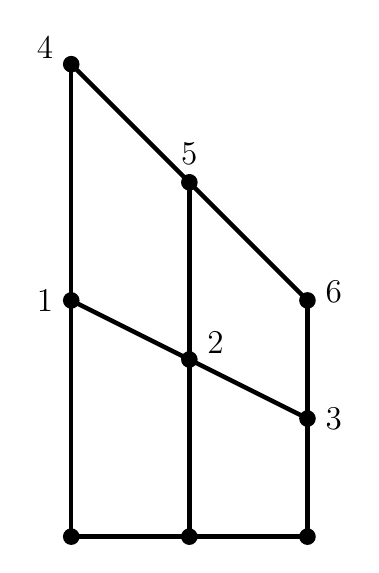
\begin{tikzpicture}
% coordinates
\coordinate (SW) at ( 0.5, 2.5);%
\coordinate (S)  at ( 2.0, 2.5);%
\coordinate (SE) at ( 3.5, 2.5);%
\coordinate (E)  at ( 3.5, 4.0);%
\coordinate (NE) at ( 3.5, 5.5);%
\coordinate (N)  at ( 2.0, 7.0);%
\coordinate (NW) at ( 0.5, 8.5);%
\coordinate (W)  at ( 0.5, 5.5);%
\coordinate (C)  at ( 2.0, 4.75);%
% boundaries
\draw[ultra thick] (SW) -- (SE);
\draw[ultra thick] (SE) -- (NE);
\draw[ultra thick] (NE) -- (NW);
\draw[ultra thick] (NW) -- (SW);
% gridlines
\draw[ultra thick] (S) -- (N);
\draw[ultra thick] (E) -- (W);
% nodes
\fill (SW) circle (3pt);
\fill (S)  circle (3pt);
\fill (SE) circle (3pt);
\fill (E)  circle (3pt) node [right=3pt,font=\large]           {$3$};	
\fill (NE) circle (3pt) node [above=3pt,right=3pt,font=\large] {$6$};
\fill (N)  circle (3pt) node [above=3pt,font=\large]           {$5$};
\fill (NW) circle (3pt) node [above=6pt,left=3pt,font=\large]  {$4$};
\fill (W)  circle (3pt) node [left=3pt,font=\large]            {$1$};	
\fill (C)  circle (3pt) node [above=6pt,right=3pt,font=\large] {$2$};	
\end{tikzpicture}
\subcaption{Structured numbering}
\label{fig:figures-bandwidth-structured}
\end{minipage}
\hfill
\begin{minipage}[t]{0.49\textwidth}
\centering
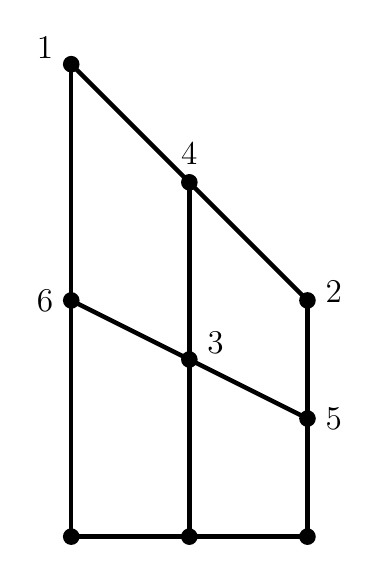
\begin{tikzpicture}
% coordinates
\coordinate (SW) at ( 0.5, 2.5);%
\coordinate (S)  at ( 2.0, 2.5);%
\coordinate (SE) at ( 3.5, 2.5);%
\coordinate (E)  at ( 3.5, 4.0);%
\coordinate (NE) at ( 3.5, 5.5);%
\coordinate (N)  at ( 2.0, 7.0);%
\coordinate (NW) at ( 0.5, 8.5);%
\coordinate (W)  at ( 0.5, 5.5);%
\coordinate (C)  at ( 2.0, 4.75);%
% boundaries
\draw[ultra thick] (SW) -- (SE);
\draw[ultra thick] (SE) -- (NE);
\draw[ultra thick] (NE) -- (NW);
\draw[ultra thick] (NW) -- (SW);
% gridlines
\draw[ultra thick] (S) -- (N);
\draw[ultra thick] (E) -- (W);
% nodes
\fill (SW) circle (3pt);
\fill (S)  circle (3pt);
\fill (SE) circle (3pt);
\fill (E)  circle (3pt) node [right=3pt,font=\large]           {$5$};	
\fill (NE) circle (3pt) node [above=3pt,right=3pt,font=\large] {$2$};
\fill (N)  circle (3pt) node [above=3pt,font=\large]           {$4$};
\fill (NW) circle (3pt) node [above=6pt,left=3pt,font=\large]  {$1$};
\fill (W)  circle (3pt) node [left=3pt,font=\large]            {$6$};	
\fill (C)  circle (3pt) node [above=6pt,right=3pt,font=\large] {$3$};	
\end{tikzpicture}
\subcaption{Random numbering}
\label{fig:figures-bandwidth-random}
\end{minipage}
\caption{Global equation numbering of nodes for structured and random node numbering.}
\label{fig:figures-bandwidth}
\end{figure}

\begin{figure}[!ht]
\centering
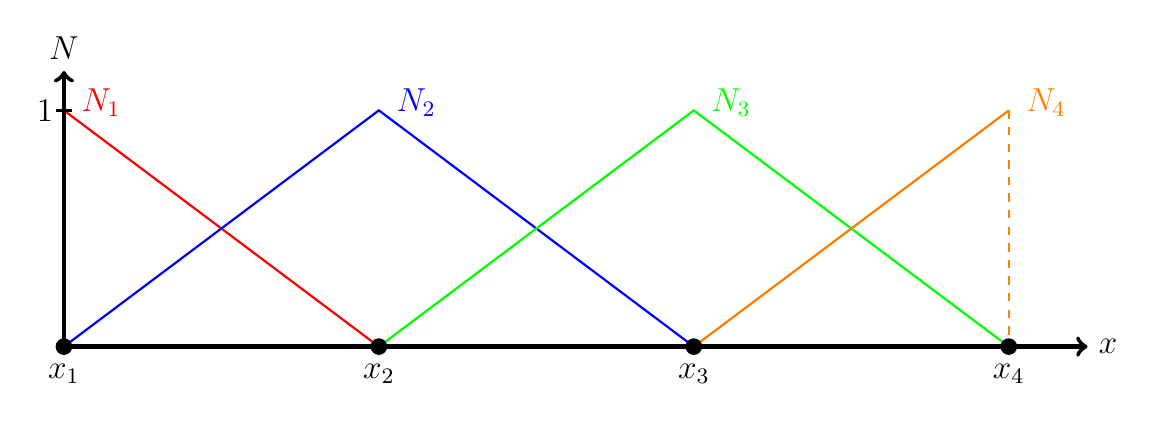
\begin{tikzpicture}
%width=15.91774cm
%height=23.56227cm
% coordinates
\coordinate (origin) at ( 0.5, 2.5);
\coordinate (xaxis)  at (13.5, 2.5);
\coordinate (Naxis)  at ( 0.5, 6.0);
\coordinate (x1)     at ( 0.5, 2.5);
\coordinate (x2)     at ( 4.5, 2.5);
\coordinate (x3)     at ( 8.5, 2.5);
\coordinate (x4)     at (12.5, 2.5);
\coordinate (N1a)    at ( 0.5, 5.5);
\coordinate (N1b)    at ( 4.5, 2.5);
\coordinate (N2a)    at ( 0.5, 2.5);
\coordinate (N2b)    at ( 4.5, 5.5);
\coordinate (N2c)    at ( 8.5, 2.5);
\coordinate (N3a)    at ( 4.5, 2.5);
\coordinate (N3b)    at ( 8.5, 5.5);
\coordinate (N3c)    at (12.5, 2.5);
\coordinate (N4a)    at ( 8.5, 2.5);
\coordinate (N4b)    at (12.5, 5.5);
% shape functions
\draw[thick,-,red]    (N1a) -- (N1b);
\draw ( 0.6,5.3) node[anchor=south west,color=red,font=\large] {$N_{1}$};
\draw[thick,-,blue]   (N2a) -- (N2b) -- (N2c);
\draw ( 4.6,5.3) node[anchor=south west,color=blue,font=\large] {$N_{2}$};
\draw[thick,-,green]  (N3a) -- (N3b) -- (N3c);
\draw ( 8.6,5.3) node[anchor=south west,color=green,font=\large] {$N_{3}$};
\draw[thick,-,orange] (N4a) -- (N4b);
\draw[thick,dashed,orange] (N4b) -- (x4);
\draw (12.6,5.3) node[anchor=south west,color=orange,font=\large] {$N_{4}$};
% axes
\draw[ultra thick,->] (origin) -- (xaxis) node[anchor=west,font=\large] {$x$};
\draw[ultra thick,->] (origin) -- (Naxis) node[anchor=south,font=\large] {$N$};
% nodes
\draw[thick,-] (0.4,5.5) -- (0.6,5.5) node [left=3pt,font=\large] {$1$};
\fill (x1) circle (3pt) node [below=3pt,font=\large] {$x_{1}$};
\fill (x2) circle (3pt) node [below=3pt,font=\large] {$x_{2}$};
\fill (x3) circle (3pt) node [below=3pt,font=\large] {$x_{3}$};
\fill (x4) circle (3pt) node [below=3pt,font=\large] {$x_{4}$};	
\end{tikzpicture}
\caption{Linear shape functions on the global domain for $n=3$.}
\label{fig:figures-shape-functions}
\end{figure}

\begin{figure}[!ht]
\centering
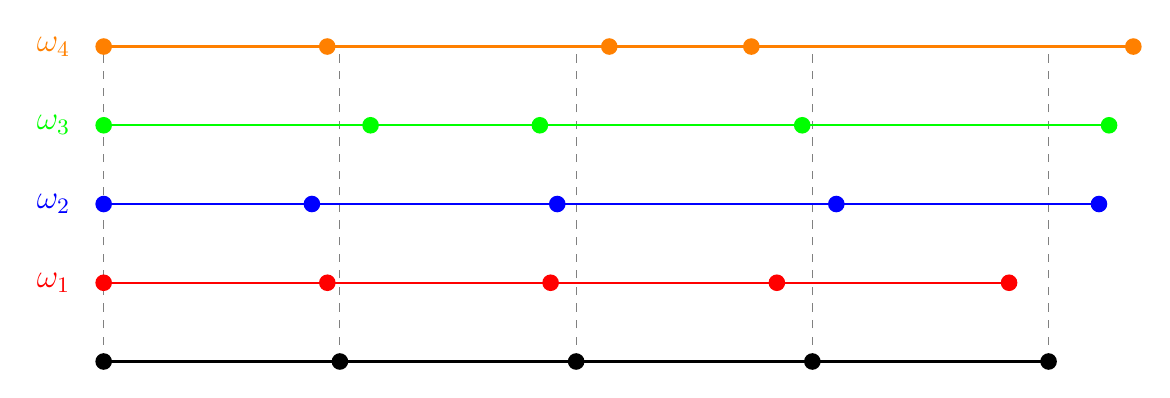
\begin{tikzpicture}
%width=15.91774cm
%height=23.56227cm
% coordinates
\coordinate (xA1) at ( 0.50      , 2.5);
\coordinate (xA2) at ( 3.50      , 2.5);
\coordinate (xA3) at ( 6.50      , 2.5);
\coordinate (xA4) at ( 9.50      , 2.5);
\coordinate (xA5) at (12.50      , 2.5);
\coordinate (xB1) at ( 0.50      , 3.5);
\coordinate (xB2) at ( 3.5-0.1598, 3.5);
\coordinate (xB3) at ( 6.5-0.3242, 3.5);
\coordinate (xB4) at ( 9.5-0.4509, 3.5);
\coordinate (xB5) at (12.5-0.5019, 3.5);
\coordinate (xC1) at ( 0.50      , 4.5);
\coordinate (xC2) at ( 3.5-0.3556, 4.5);
\coordinate (xC3) at ( 6.5-0.2396, 4.5);
\coordinate (xC4) at ( 9.5+0.3041, 4.5);
\coordinate (xC5) at (12.5+0.6401, 4.5);
\coordinate (xD1) at ( 0.50      , 5.5);
\coordinate (xD2) at ( 3.5+0.3892, 5.5);
\coordinate (xD3) at ( 6.5-0.4606, 5.5);
\coordinate (xD4) at ( 9.5-0.1286, 5.5);
\coordinate (xD5) at (12.5+0.7683, 5.5);
\coordinate (xE1) at ( 0.50      , 6.5);
\coordinate (xE2) at ( 3.5-0.1610, 6.5);
\coordinate (xE3) at ( 6.5+0.4209, 6.5);
\coordinate (xE4) at ( 9.5-0.7748, 6.5);
\coordinate (xE5) at (12.5+1.0765, 6.5);
\coordinate (xZ1) at ( 0.50      , 6.5);
\coordinate (xZ2) at ( 3.50      , 6.5);
\coordinate (xZ3) at ( 6.50      , 6.5);
\coordinate (xZ4) at ( 9.50      , 6.5);
\coordinate (xZ5) at (12.50      , 6.5);
% shape functions
\draw[thin,dashed,gray] (xA1) -- (xZ1);
\draw[thin,dashed,gray] (xA2) -- (xZ2);
\draw[thin,dashed,gray] (xA3) -- (xZ3);
\draw[thin,dashed,gray] (xA4) -- (xZ4);
\draw[thin,dashed,gray] (xA5) -- (xZ5);
\draw[thick,-,black]  (xA1) -- (xA2) -- (xA3) -- (xA4) -- (xA5);
\fill[black]  (xA1) circle (3pt);
\fill[black]  (xA2) circle (3pt);
\fill[black]  (xA3) circle (3pt);
\fill[black]  (xA4) circle (3pt);
\fill[black]  (xA5) circle (3pt);
\draw[thick,-,red]    (xB1) -- (xB2) -- (xB3) -- (xB4) -- (xB5);
\draw (xB1) node[anchor=east,left=3mm,color=red,font=\large] {$\omega_{1}$~};
\fill[red]    (xB1) circle (3pt);
\fill[red]    (xB2) circle (3pt);
\fill[red]    (xB3) circle (3pt);
\fill[red]    (xB4) circle (3pt);
\fill[red]    (xB5) circle (3pt);
\draw[thick,-,blue]   (xC1) -- (xC2) -- (xC3) -- (xC4) -- (xC5);
\draw (xC1) node[anchor=east,left=3mm,color=blue,font=\large] {$\omega_{2}$~};
\fill[blue]   (xC1) circle (3pt);
\fill[blue]   (xC2) circle (3pt);
\fill[blue]   (xC3) circle (3pt);
\fill[blue]   (xC4) circle (3pt);
\fill[blue]   (xC5) circle (3pt);
\draw[thick,-,green]  (xD1) -- (xD2) -- (xD3) -- (xD4) -- (xD5);
\draw (xD1) node[anchor=east,left=3mm,color=green,font=\large] {$\omega_{3}$~};
\fill[green]  (xD1) circle (3pt);
\fill[green]  (xD2) circle (3pt);
\fill[green]  (xD3) circle (3pt);
\fill[green]  (xD4) circle (3pt);
\fill[green]  (xD5) circle (3pt);
\draw[thick,-,orange] (xE1) -- (xE2) -- (xE3) -- (xE4) -- (xE5);
\draw (xE1) node[anchor=east,left=3mm,color=orange,font=\large] {$\omega_{4}$~};
\fill[orange] (xE1) circle (3pt);
\fill[orange] (xE2) circle (3pt);
\fill[orange] (xE3) circle (3pt);
\fill[orange] (xE4) circle (3pt);
\fill[orange] (xE5) circle (3pt);
\end{tikzpicture}
\caption{Mode shapes for $n=4$.}
\label{fig:figures-mode-shapes}
\end{figure}
